\documentclass[11pt,a4paper]{article}

% ── FONTS ────────────────────────────────────────────────────
\usepackage{fontspec}
\setmainfont{Calibri}
\setsansfont{Calibri}
\newfontfamily{\hindifont}{Nirmala UI}[Script=Devanagari]
\newcommand{\hindi}[1]{{\hindifont #1}}

% ── LAYOUT ───────────────────────────────────────────────────
\usepackage[top=2cm,bottom=2.5cm,left=2.2cm,right=2.2cm]{geometry}
\usepackage{graphicx}
\usepackage{xcolor}
\usepackage{tikz}
\usetikzlibrary{calc}
\usepackage{tcolorbox}
\tcbuselibrary{skins,breakable}
\usepackage{colortbl}
\usepackage{booktabs}
\usepackage{tabularx}
\usepackage{enumitem}
\usepackage{setspace}
\usepackage{fancyhdr}
\usepackage{titlesec}
\usepackage{hanging}
\usepackage{multicol}
\usepackage{xurl}
\usepackage{hyperref}
\usepackage{microtype}
\usepackage{array}
\usepackage{caption}

\hypersetup{colorlinks=false,hidelinks,breaklinks=true,unicode=true}

% ── BRAND COLORS ────────────────────────────────────────────
\definecolor{navyblue}{HTML}{003566}
\definecolor{gold}{HTML}{C9A84C}
\definecolor{lightgray}{HTML}{F4F6FB}
\definecolor{midgray}{HTML}{D0D6E2}
\definecolor{darkgray}{HTML}{4A4A4A}
\definecolor{accentteal}{HTML}{0077B6}
\definecolor{sectionbg}{HTML}{EEF2FA}

% ── SECTION HEADING COMMAND ──────────────────────────────────
% titlesec passes the section title as argument to the last command
% in before-code if it takes a mandatory argument
\newcommand{\navysectionbox}[1]{%
  \hspace{-2.2cm}%
  \colorbox{navyblue}{%
    \hspace{2.2cm}%
    \parbox[c][0.65cm]{\dimexpr\textwidth+2.0cm-2pt\relax}{%
      \raggedright
      {\fontsize{12}{14}\selectfont\color{white}\strut\textbf{#1}}%
    }%
  }%
}

\titleformat{\section}[block]
  {\normalfont}
  {}{0em}
  {\navysectionbox}
\titlespacing*{\section}{-2.2cm}{16pt}{8pt}

\titleformat{\subsection}[block]
  {\normalfont\bfseries\fontsize{10.5}{13}\selectfont\color{navyblue}}
  {}{0em}{}
\titlespacing*{\subsection}{0pt}{10pt}{2pt}

% ── HEADER / FOOTER ─────────────────────────────────────────
\setlength{\headheight}{20pt}
\pagestyle{fancy}
\fancyhf{}
\fancyhead[L]{\footnotesize\color{navyblue}\textbf{AIGGPA Bhopal} \quad\textbar\quad
  IT Utilisation Assessment}
\fancyhead[R]{\footnotesize\color{navyblue}April 2026}
\fancyfoot[C]{\footnotesize\color{navyblue}\thepage}
\renewcommand{\headrulewidth}{0.4pt}
\renewcommand{\headrule}{\color{navyblue}\hrule width\headwidth height\headrulewidth}
\renewcommand{\footrulewidth}{1.5pt}
\renewcommand{\footrule}{\color{gold}\hrule width\headwidth height 1.5pt}

% ── CUSTOM BOXES ────────────────────────────────────────────
\newtcolorbox{goldbox}{
  colback=gold!10, colframe=gold, boxrule=0.7pt, arc=3mm,
  left=10pt, right=10pt, top=8pt, bottom=8pt, breakable
}

\newtcolorbox{navybox}{
  colback=sectionbg, colframe=navyblue, boxrule=0.6pt, arc=3mm,
  left=10pt, right=10pt, top=8pt, bottom=8pt, breakable
}

\newtcolorbox{streamboxa}{
  colback=lightgray, colframe=accentteal, boxrule=1.2pt, arc=3mm,
  lefttitle=8pt, toptitle=4pt, bottomtitle=4pt,
  left=8pt, right=8pt, top=6pt, bottom=6pt,
  title={\bfseries\fontsize{9}{11}\selectfont\color{white}
    Stream A \textbullet{} Department Officials},
  colbacktitle=accentteal, breakable
}

\newtcolorbox{streamboxb}{
  colback=lightgray, colframe=navyblue, boxrule=1.2pt, arc=3mm,
  lefttitle=8pt, toptitle=4pt, bottomtitle=4pt,
  left=8pt, right=8pt, top=6pt, bottom=6pt,
  title={\bfseries\fontsize{9}{11}\selectfont\color{white}
    Stream B \textbullet{} IT Department},
  colbacktitle=navyblue, breakable
}

% ── LISTS ───────────────────────────────────────────────────
\setlist[itemize]{leftmargin=1.2em, itemsep=2pt, topsep=3pt}
\setlist[enumerate]{leftmargin=1.4em, itemsep=2pt, topsep=3pt}

% Allow extra stretch so long words / URLs wrap without huge overfull boxes
\setlength{\emergencystretch}{2.5em}

% ────────────────────────────────────────────────────────────
\begin{document}
\onehalfspacing

% ════════════════════════════════════════════════════════════
%  COVER PAGE
% ════════════════════════════════════════════════════════════
\thispagestyle{empty}
\begin{tikzpicture}[remember picture, overlay]
  \fill[navyblue] (current page.south west) rectangle (current page.north east);
  \fill[gold] (current page.south west)
    rectangle ($(current page.south east)+(0,1.1cm)$);
  \fill[white] ($(current page.south west)+(0,1.1cm)$)
    rectangle ($(current page.south east)+(0,11.8cm)$);
  \fill[accentteal!80]
    ($(current page.south west)+(0,11.8cm)$) --
    ($(current page.south east)+(0,11.8cm)$) --
    ($(current page.south east)+(0,13.2cm)$) --
    ($(current page.south west)+(0,12.4cm)$) -- cycle;
\end{tikzpicture}

\vspace*{6cm}
\begin{center}
  \fontsize{8.5}{10}\selectfont\color{gold!80}
  \textbf{\MakeUppercase{Research Proposal \textbullet{} Internship 2026}}\\[0.7em]
  \fontsize{26}{31}\selectfont\bfseries\color{white}
  Assessment of IT Tool\\[0.15em]
  Utilisation Among\\[0.15em]
  Government Officials\\[0.9em]
  \fontsize{11}{14}\selectfont\color{midgray}
  \hindi{सरकारी अधिकारियों द्वारा आईटी उपकरणों के उपयोग का आकलन}
\end{center}

\vspace*{2.5cm}
\begin{tikzpicture}[remember picture, overlay]
  \node[anchor=south west] at ($(current page.south west)+(2.2cm,1.5cm)$){%
    \begin{minipage}{14cm}
      \footnotesize\color{darkgray}
      \begin{tabular}{@{}ll@{}}
        \textbf{Submitted by:}   & Aryan Kori, Summer Intern 2026 \\[3pt]
        \textbf{Institution:}    & AIGGPA, Bhopal \\[3pt]
        \textbf{Departments:}    & School Education \textbullet{}
                                   Health \textbullet{}
                                   Forest, Govt. of MP \\[3pt]
        \textbf{Date:}           & April 2026 \\
      \end{tabular}
    \end{minipage}%
  };
\end{tikzpicture}

\newpage

% ════════════════════════════════════════════════════════════
%  EXECUTIVE SUMMARY
% ════════════════════════════════════════════════════════════
\begin{goldbox}
  \textbf{\color{navyblue}\large Executive Summary}\\[6pt]
  Madhya Pradesh has invested heavily in digital portals like Education Portal 3.0, e-Office, and HRMIS. But during my initial observations, I noticed a huge gap: district and block officials still rely heavily on paper, WhatsApp, and Excel instead of the official platforms. 
  
  This proposal outlines a quick field study to find out exactly \textit{what} tools our officials are actually using, \textit{why} they avoid the official platforms, and how AIGGPA can step in to train them better.
\end{goldbox}

\vspace{0.4cm}

% ════════════════════════════════════════════════════════════
%  BACKGROUND
% ════════════════════════════════════════════════════════════
\section{Background}

\vspace{0.2cm}
I looked into three major departments to understand the scale of the tools they currently have available:
\begin{itemize}[leftmargin=1.4em]
  \item \textbf{School Education}: They run the Education Portal 3.0 (Figure~1), which is supposed to manage everything for roughly 350,000 permanent teachers across more than 92,000 schools.\footnote{Teacher workforce scale is used here as contextual background only, corroborated against independent press reporting (Free Press Journal, n.d.); see References.}
  \item \textbf{Health}: They operate HRMIS, NHM CHETNA for frontline workers, and have launched an AI-assisted chatbot, ``Ayushman Sakhi,'' positioned to help users locate hospitals and related services.\footnote{Chatbot launch and features are described in general-audience reporting (India.com News Desk, 2025). NTEP portal materials cited for broader health ICT context (National Tuberculosis Elimination Programme, n.d.); see References.}
  \item \textbf{Forest}: The department reports AI-assisted, near real-time forest alert capabilities linked to satellite analytics, alongside routine processing of wildlife tourism services through MPOnline.\footnote{Reporting on the state's AI-based forest alert initiative (The Indian Express, 2024). Forest department online service channel (Government of Madhya Pradesh, n.d.); see References.}
\end{itemize}

\begin{figure}[htbp]
\centering
\setlength{\fboxsep}{0pt}\setlength{\fboxrule}{0.8pt}%
\fcolorbox{navyblue}{white}{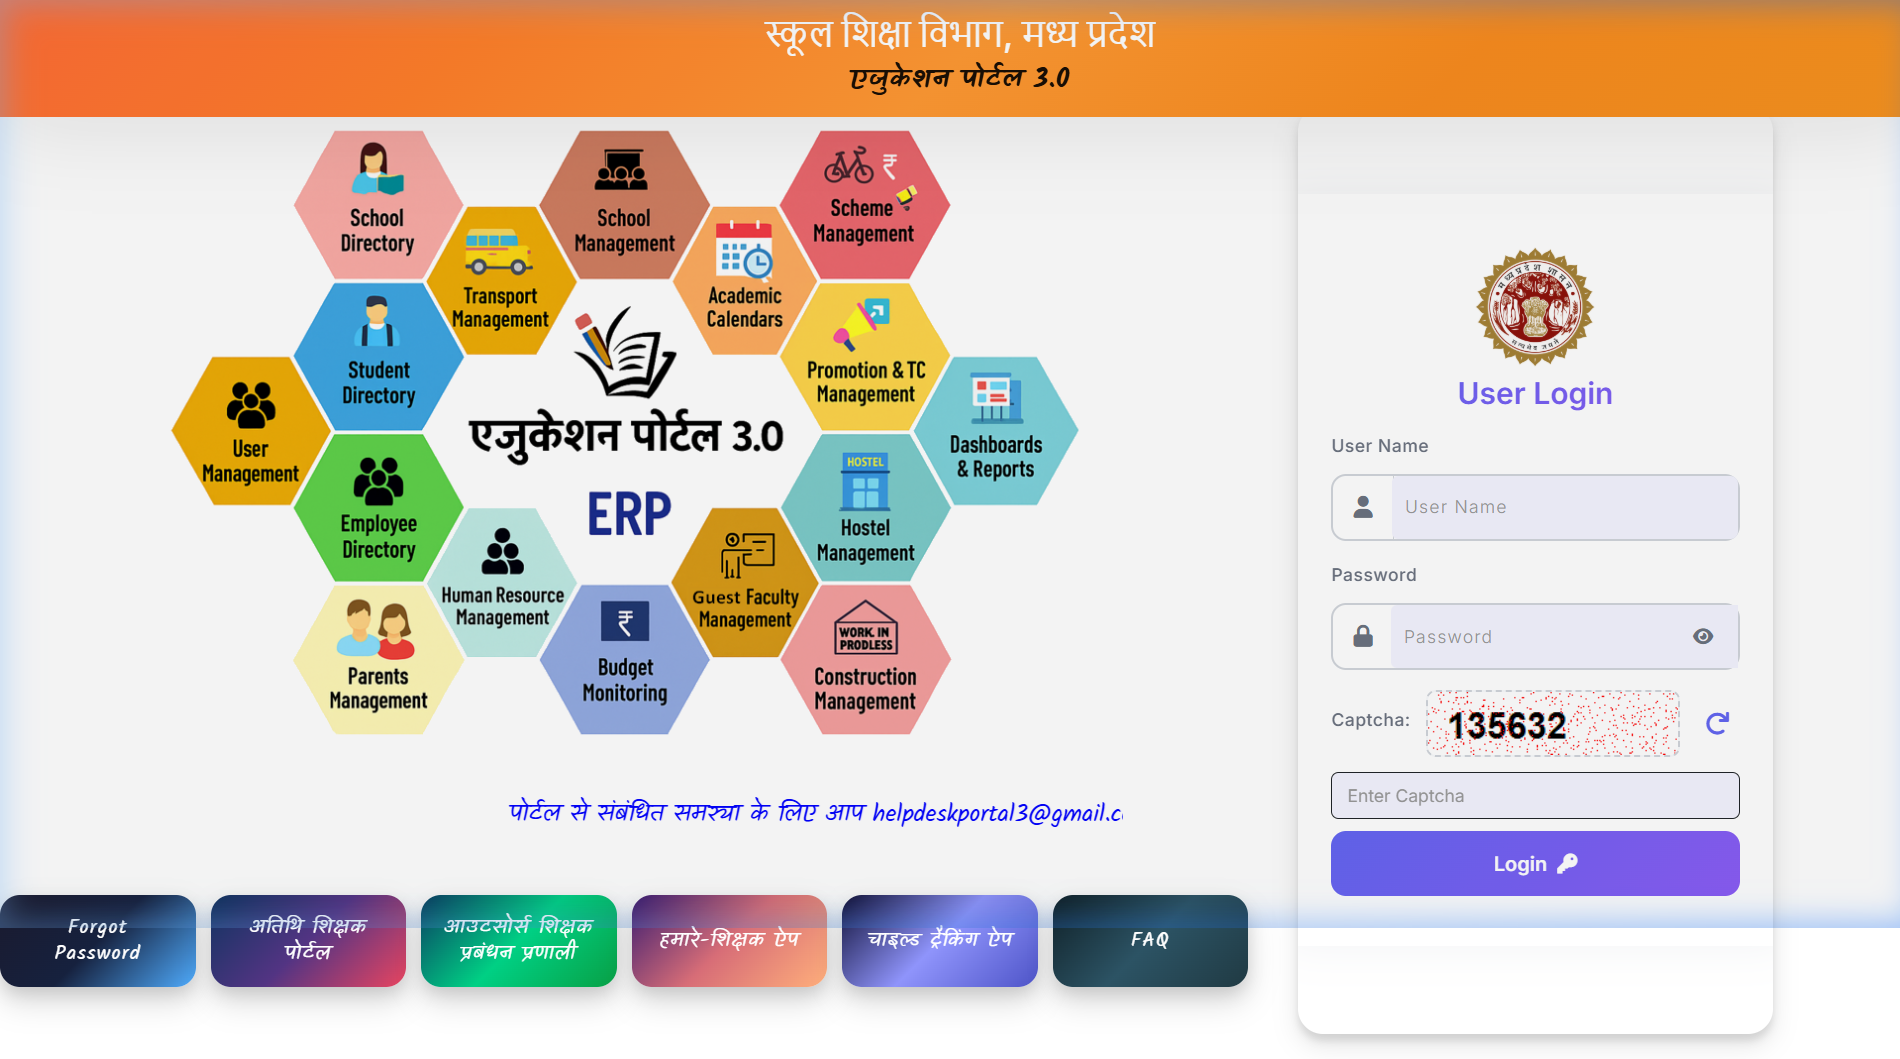
\includegraphics[width=0.85\textwidth]{figures/fig3_education_portal.png}}
\vspace{0.1cm}
\caption{\small\textit{\textbf{Figure 1.} MP Education Portal 3.0 showing twelve integrated management modules.
  School Education Department, Government of Madhya Pradesh (2025).\protect\footnotemark}}
\end{figure}
\footnotetext{Official portal description and access point (Government of Madhya Pradesh, School Education Department, 2025); see References.}

Despite these massive systems being built and paid for, local officials often ignore them. They stick to physical registers and physical dak. This study simply asks: who is actually using what, and why is there such a roadblock?

% ════════════════════════════════════════════════════════════
%  RESEARCH OBJECTIVES
% ════════════════════════════════════════════════════════════
\section{Research Objectives}

\vspace{0.2cm}
\begin{navybox}
\begin{enumerate}[label={\color{gold}\bfseries\arabic*.},itemsep=4pt]
  \item Find out what tools officials are \textbf{actually using} (both official platforms and informal ones like WhatsApp).
  \item See how they process their daily files and type their letters.
  \item Talk to the IT department to get their side of the story on why adoption is low.
  \item Group the roadblocks into the five \textbf{SAAMP} dimensions: \textbf{S}kill, \textbf{A}wareness, \textbf{A}vailability, \textbf{M}otivation, and \textbf{P}rocess.
\end{enumerate}
\end{navybox}

% ════════════════════════════════════════════════════════════
%  SCOPE
% ════════════════════════════════════════════════════════════
\section{Scope}

\vspace{0.2cm}
\renewcommand{\arraystretch}{1.45}
\begin{tabularx}{\textwidth}{%
  >{\columncolor{navyblue}\color{white}\bfseries\small}p{3.2cm}%
  >{\columncolor{lightgray}\small}X}
Departments & School Education \textbullet{} Health \textbullet{}
             Forest (Government of Madhya Pradesh) \\
\rowcolor{white}
Respondents & Department officials (Class I, II, III) and IT cell / IT dept. staff \\
\rowcolor{lightgray}
Office Level & State level (Bhopal) and district offices, subject to access \\
\rowcolor{white}
Duration & April to June 2026 \\
\rowcolor{lightgray}
Output & Gap analysis report and recommendations for AIGGPA \\
\end{tabularx}

% ════════════════════════════════════════════════════════════
%  METHODOLOGY
% ════════════════════════════════════════════════════════════
\section{Methodology}

\vspace{0.2cm}

This study uses a \textbf{qualitative, exploratory} design suited to understanding everyday practice in government offices. Semi-structured interviews and short structured prompts will capture \textit{what} tools are used, \textit{how} work flows between people and systems, and \textit{why} certain platforms are preferred or avoided. The framing draws on technology acceptance research (e.g.\ perceived usefulness and ease of use; Davis, 1989) and on the idea that adoption depends on organisational context and process, not only on software features (Tornatzky \& Fleischer, 1990). Mission Karmayogi's emphasis on role-based capacity building (Government of India, DoPT, 2020) aligns with translating findings into training rather than blame.

\subsection{Participants and sampling}

Officials in School Education, Health, and Forest will be approached at \textbf{state level (Bhopal)} and, where access permits, at \textbf{district} offices. Sampling will be \textbf{purposive}: respondents are chosen because they routinely handle files, data entry, or coordination---typically Class I--III officers and equivalent staff, plus IT cell or IT department representatives. Numbers will depend on gatekeeping and time; the aim is \textbf{saturation} on recurring themes per department rather than a fixed $n$. All participation will be voluntary; roles and departments may be anonymised in reporting if requested.

\subsection{Data collection}

To get the full picture, I will engage two complementary streams (Figure~2):

\vspace{0.2cm}
\begin{figure}[htbp]
\centering
\setlength{\fboxsep}{0pt}\setlength{\fboxrule}{0.8pt}%
\fcolorbox{navyblue}{white}{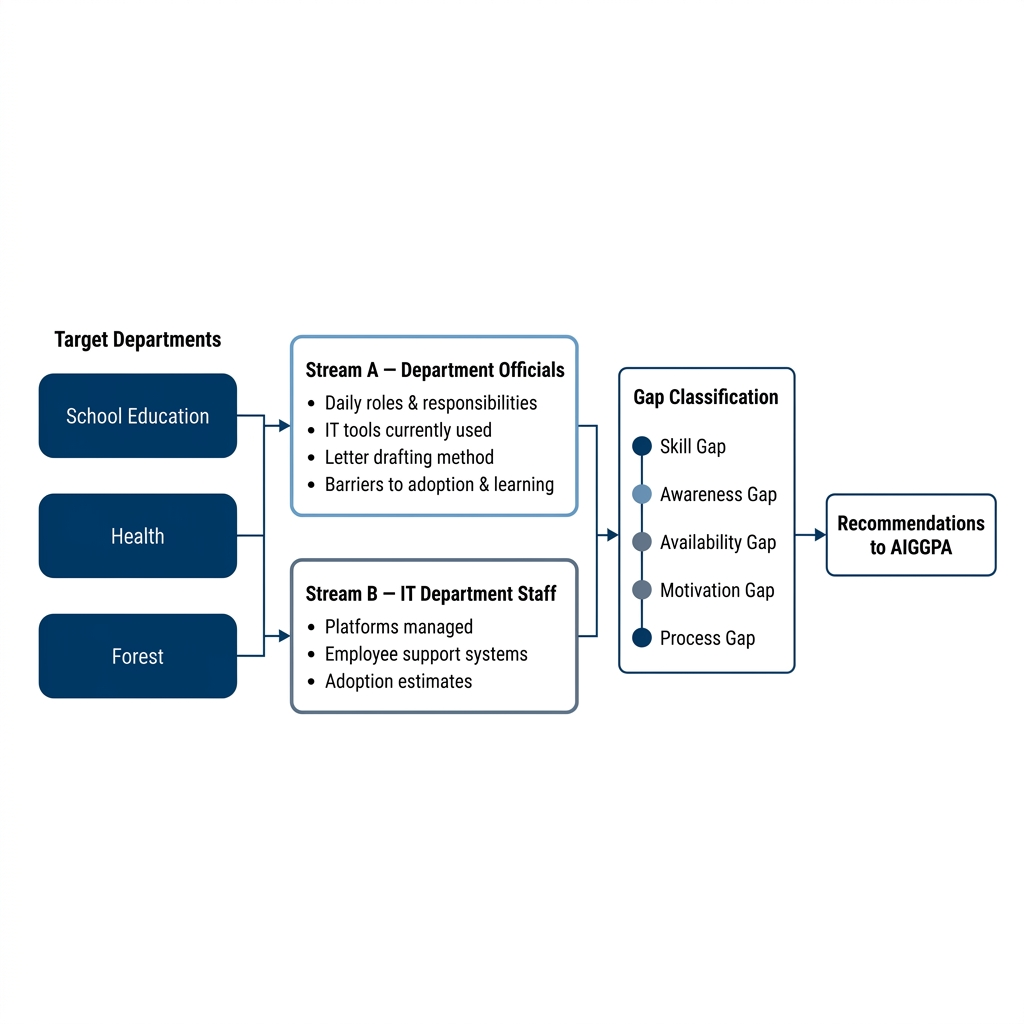
\includegraphics[width=0.85\textwidth]{figures/fig1_research_design.png}}
\vspace{0.1cm}
\caption{\small\textit{\textbf{Figure 2.} Research design: three departments, two
  data collection streams, gap classification, and AIGGPA recommendations.}}
\end{figure}

\vspace{0.3cm}
\begin{multicols}{2}

\begin{streamboxa}
\small
\begin{itemize}[leftmargin=1em,itemsep=2pt,topsep=2pt]
  \item What tasks do you do every day?
  \item Which apps or websites do you use to do them?
  \item Why don't you use the official portal?
  \item Who taught you how to use your current tools?
\end{itemize}
\end{streamboxa}

\columnbreak

\begin{streamboxb}
\small
\begin{itemize}[leftmargin=1em,itemsep=2pt,topsep=2pt]
  \item What tools have you built for the staff?
  \item How many people actually log in?
  \item What do you think is stopping them?
  \item How do you handle tech support?
\end{itemize}
\end{streamboxb}

\end{multicols}

\vspace{0.3cm}

\begin{figure}[htbp]
\centering
\setlength{\fboxsep}{0pt}\setlength{\fboxrule}{0.8pt}%
\fcolorbox{navyblue}{white}{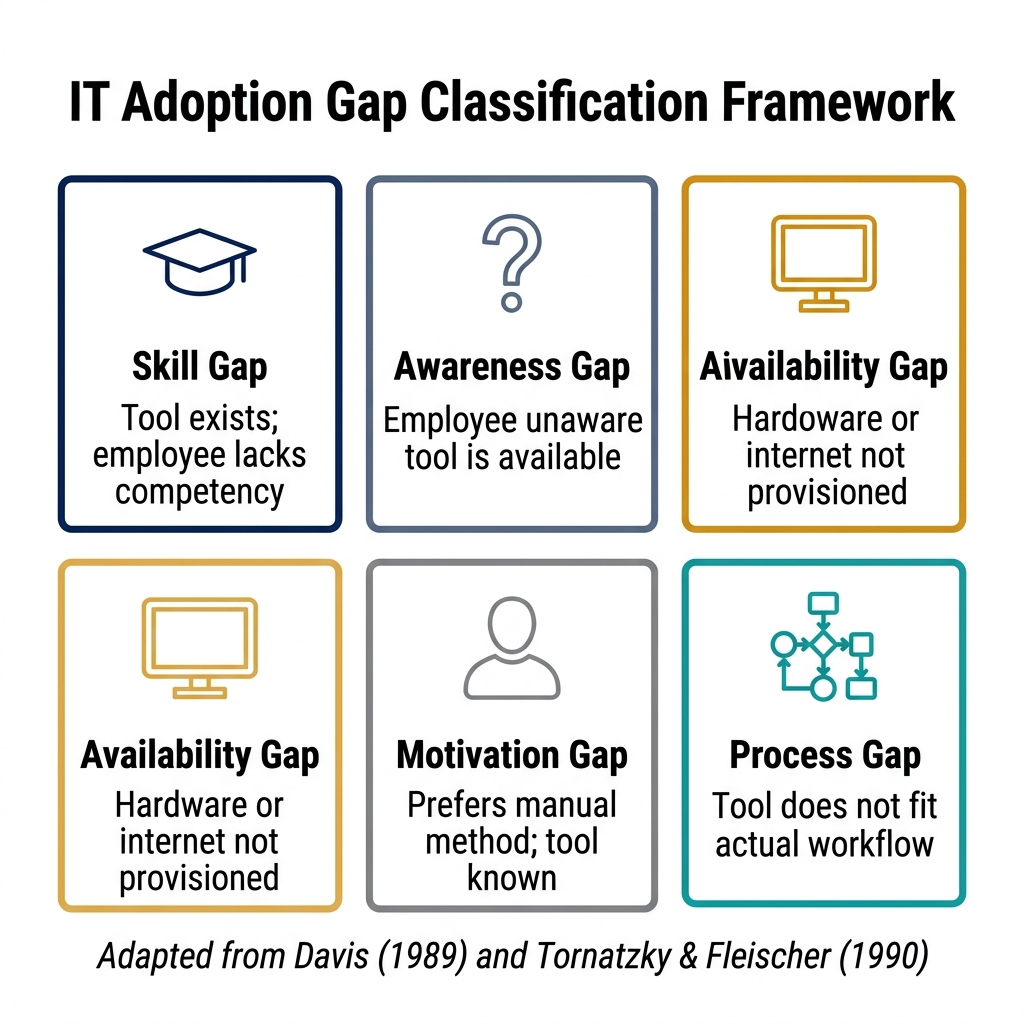
\includegraphics[width=0.85\textwidth]{figures/fig2_gap_classification.png}}
\vspace{0.1cm}
\caption{\small\textit{\textbf{Figure 3.} SAAMP gap taxonomy (Skill, Awareness, Availability, Motivation, Process).}}
\end{figure}

\vspace{0.3cm}

\noindent\textbf{Stream A} uses a short interview guide (see box) to record tasks, tools, workarounds, and training history. \textbf{Stream B} captures deployment metrics where shareable (e.g.\ login trends, help-desk load), perceived barriers from the IT side, and support processes. Where ethical and practical, I may note \textbf{observable} patterns (e.g.\ parallel paper trails) without collecting personal data beyond what respondents disclose in interview.

\subsection{Data Analysis Plan}

Qualitative material (verbatim transcripts where consent and logistics allow, otherwise de-identified, time-stamped field notes exported as plain text) will form a single \textbf{text corpus} per stream and department. Each document will first be normalised (standardised spelling of key platform names, segment boundaries aligned to interview questions) to support consistent processing.

\textbf{Stage 1---Computational pre-coding (Python).} The corpus will be ingested and processed in Python using established open libraries (for example \texttt{pandas} for tabular summaries, \texttt{scikit-learn} for tokenisation and weighted keyword features, and optional lightweight NLP utilities for lemmatisation or phrase detection). A controlled \textbf{SAAMP lexicon} will be defined for each dimension---Skill, Awareness, Availability, Motivation, Process---drawing on the interview guide, pilot transcripts, and prior literature. Each segment will receive \textbf{provisional SAAMP tags} based on keyword hits, cosine similarity to short ``seed'' paragraphs per category, and simple co-occurrence rules (e.g.\ connectivity + downtime $\rightarrow$ Availability). The output of this stage is a \textbf{machine-assisted codebook}: ranked candidate excerpts mapped to one or more SAAMP categories with transparent rule and score metadata.

\textbf{Stage 2---Analyst validation and integration.} A trained analyst will review every flagged excerpt and a stratified random sample of non-flagged text to correct false positives/negatives, merge duplicate themes, and attach short interpretive memos. Disagreements between computational suggestions and manual reading will be resolved in favour of context-aware judgment; ambiguous cases will be dual-coded with brief rationales. Stream~B (IT) responses will be triangulated against Stream~A to build a single \textbf{SAAMP-consistent evidence trail}.

\textbf{Stage 3---Synthesis.} Cross-tabulations by department, cadre, and office level will populate a structured \textbf{gap matrix} (tool $\times$ role $\times$ primary SAAMP barrier). Patterns that survive both computational screening and manual review feed the final recommendations. This sequence keeps the SAAMP framework fixed while combining reproducible, documented automation with qualitative rigour.

\subsection{Ethics and limitations}

No sensitive personal data will be collected beyond professional views on systems in use. Findings will be reported in aggregate with optional anonymisation. \textbf{Limitations} include restricted access to some offices, possible social desirability bias when discussing official systems, and the fact that login statistics may not be uniformly available---the design explicitly combines official and frontline perspectives to offset these gaps.

\vspace{0.35cm}

% ════════════════════════════════════════════════════════════
%  RESEARCH QUESTIONS
% ════════════════════════════════════════════════════════════
\section{Research Questions}

\vspace{0.2cm}
\begin{navybox}
\small
\begin{enumerate}[label=\textbf{RQ\arabic*.}, itemsep=6pt, leftmargin=2em]
  \item Which digital and non-digital tools do officials rely on for daily tasks, and how does this differ by department and level?
  \item What reasons along the five SAAMP dimensions best explain under-use of mandated portals and systems?
  \item How do IT departments perceive adoption, support load, and the gap between policy intent and field practice?
  \item What concrete capacity-building and process interventions can AIGGPA recommend, prioritised by feasibility and impact?
\end{enumerate}
\end{navybox}

% ════════════════════════════════════════════════════════════
%  SIGNIFICANCE
% ════════════════════════════════════════════════════════════
\section{Significance}

\vspace{0.2cm}
Madhya Pradesh has invested in large-scale digital platforms; low utilisation wastes public investment and slows service delivery. A clear, evidence-backed picture of \textit{actual} use versus \textit{official} tools helps AIGGPA target training, change management, and handholding where they matter---aligned with national capacity-building direction---rather than generic IT literacy. The three departments chosen differ in citizen touchpoints and technology maturity, which should yield transferable lessons for other line departments.

% ════════════════════════════════════════════════════════════
%  WORK PLAN
% ════════════════════════════════════════════════════════════
\section{Work Plan (April--June 2026)}

\vspace{0.2cm}
\renewcommand{\arraystretch}{1.4}
\begin{tabularx}{\textwidth}{%
  >{\columncolor{navyblue}\color{white}\bfseries\small}p{2.6cm}%
  >{\columncolor{lightgray}\small}X}
Weeks 1--2 &
Literature and document scan; finalise guides; confirm access and respondents with AIGGPA and departments. \\
\rowcolor{white}
Weeks 3--6 &
Field interviews (Streams A and B); contemporaneous notes; optional follow-up calls for clarification. \\
\rowcolor{lightgray}
Weeks 7--8 &
Python-assisted SAAMP pre-coding, manual validation, utilisation map and gap matrix; draft recommendations. \\
\rowcolor{white}
Weeks 9--10 &
Internal review at AIGGPA; revise report; final presentation / handover of deliverables. \\
\end{tabularx}

% ════════════════════════════════════════════════════════════
%  AUDIT TRAIL
% ════════════════════════════════════════════════════════════
\section{Research Notes \& Sources}

\vspace{0.2cm}
\noindent External quantitative and programme claims used for \textit{background context only} were checked against publicly available news and official portal pages before drafting.\footnote{Teacher-scale context (Free Press Journal, n.d.).}\footnote{Ayushman Sakhi launch (India.com News Desk, 2025); health portal context (National Tuberculosis Elimination Programme, n.d.).}\footnote{Forest AI alert reporting (The Indian Express, 2024); forest e-services channel (Government of Madhya Pradesh, n.d.).} Full bibliographic entries and URLs appear in \textbf{References}.

% ════════════════════════════════════════════════════════════
%  EXPECTED OUTPUT
% ════════════════════════════════════════════════════════════
\section{Expected Output}

\vspace{0.2cm}
\noindent The internship will produce one consolidated \textbf{gap analysis report} for AIGGPA, plus slides or a short briefing note suitable for department stakeholders. Deliverables below summarise the structure of that report.

\vspace{0.25cm}
\begin{multicols}{3}

\begin{tcolorbox}[colback=navyblue,colframe=navyblue,arc=4mm,
  left=8pt,right=8pt,top=8pt,bottom=8pt]
\centering
{\color{gold}\bfseries\large 01}\\[4pt]
{\color{white}\small\textbf{IT Utilisation Map}\\[4pt]
Role-wise and level-wise map of tools used vs. available}
\end{tcolorbox}

\columnbreak

\begin{tcolorbox}[colback=accentteal,colframe=accentteal,arc=4mm,
  left=8pt,right=8pt,top=8pt,bottom=8pt]
\centering
{\color{white}\bfseries\large 02}\\[4pt]
{\color{white}\small\textbf{Gap Analysis Matrix}\\[4pt]
Gaps classified by department, level, and gap type}
\end{tcolorbox}

\columnbreak

\begin{tcolorbox}[colback=gold,colframe=gold,arc=4mm,
  left=8pt,right=8pt,top=8pt,bottom=8pt]
\centering
{\color{navyblue}\bfseries\large 03}\\[4pt]
{\color{navyblue}\small\textbf{AIGGPA Recommendations}\\[4pt]
Targeted capacity building interventions}
\end{tcolorbox}

\end{multicols}

\vspace{0.35cm}
\noindent\small\textit{Optional stretch goal:} a one-page ``quick wins'' annex (e.g.\ refresher modules, SOP hints, help-desk triage) if time and department feedback allow.

% ════════════════════════════════════════════════════════════
%  CONCLUSION
% ════════════════════════════════════════════════════════════
\section{Conclusion}

\vspace{0.2cm}
This proposal sets out a focused, feasible study of IT tool utilisation across three major departments, using dual streams of field and IT perspectives and the \textbf{SAAMP} gap taxonomy. Results will feed directly into AIGGPA's mandate for training and administrative improvement and support evidence-led digital governance in Madhya Pradesh.

% ════════════════════════════════════════════════════════════
%  REFERENCES
% ════════════════════════════════════════════════════════════
\section{References}

\vspace{0.2cm}
\begingroup
\small\setlength{\parindent}{0pt}\singlespacing\sloppy
\setlength{\emergencystretch}{4em}
\begin{hangparas}{1.27cm}{1}

Davis, F. D. (1989). Perceived usefulness, perceived ease of use, and user
acceptance of information technology. \textit{MIS Quarterly}, \textit{13}(3), 319--340.

\vspace{4pt}
Government of India, Department of Personnel \& Training. (2020).
\textit{National programme for civil services capacity building (Mission Karmayogi)}.
Ministry of Personnel, Public Grievances and Pensions.

\vspace{4pt}
Government of Madhya Pradesh, School Education Department. (2025).
\textit{Education Portal 3.0}. \url{https://sederp.educationportal3.in}

\vspace{4pt}
Tornatzky, L. G., \& Fleischer, M. (1990).
\textit{The processes of technological innovation}. Lexington Books.

\vspace{4pt}
Free Press Journal. (n.d.). MP: 3.5 lakh permanent teachers await promotions for two decades.
\textit{Free Press Journal}. \url{https://www.freepressjournal.in/bhopal/mp-35-lakh-permanent-teachers-await-promotions-for-two-decades}

\vspace{4pt}
India.com News Desk. (2025, December 12). Ayushman Sakhi: AI-based smart chatbot launched in MP.
\textit{India.com}. \url{https://www.india.com/news/india/ayushman-sakhi-ai-based-smart-chatbot-launched-in-mp-key-features-and-benefits-7140417/}

\vspace{4pt}
Indian Express. (2024, December 20). MP becomes first state to launch AI-based real-time forest alert system.
\textit{The Indian Express}. \url{https://indianexpress.com/article/india/mp-becomes-first-state-to-launch-ai-based-real-time-forest-alert-system-9273574/}

\vspace{4pt}
National Tuberculosis Elimination Programme. (n.d.). NTEP portal resources.
\url{https://ntep.in/}

\vspace{4pt}
Government of Madhya Pradesh. (n.d.). MPOnline---Forest department services.
\url{https://forest.mponline.gov.in/}

\end{hangparas}
\endgroup

\end{document}
